% !TEX TS-program = XeLaTex
% CV2 - My new curriculum vitae
%09/2022
%by: João Pereira

\documentclass[11pt,oneside,a4paper,titlepage]{article}

\usepackage[most]{tcolorbox}

\usepackage{titling}
\usepackage{titlesec}
\usepackage{multicol}
\usepackage[margin=6em]{geometry}
\usepackage{array}	%For struts
\usepackage{fontawesome5}	%For icons
\usepackage{fancyhdr}	%footers

\fancyhf{} % sets both header and footer to nothing
\renewcommand{\headrulewidth}{0pt}

\usepackage{hyperref} 	%url
\hypersetup{colorlinks=false}

%Font
\usepackage{fontspec}
\setmainfont[Ligatures=TeX]{Cambria}
\setsansfont[Ligatures=TeX]{Arial}

%  \fontencoding{T1}
 % \setmainfont{garamond}
  %\fontseries{m}
  %\fontshape{it}
  %\fontsize{12}{15}
  %\selectfont
  
%TO REMOVE
\usepackage{lipsum}


%INFO
\author{João Pereira}
\date{December 2022}

%Colors
%\definecolor{titleBack}{RGB}{0,66,21}
\definecolor{titleBack}{RGB}{255, 255, 255}
\definecolor{SecText}{RGB}{59,122,87} %Amazon green
\definecolor{textGrey}{RGB}{128, 128, 128}

%Struts
\newcolumntype{L}{>{\raggedleft}p{0.13\textwidth}}
\newcolumntype{R}{p{0.8\textwidth}}
\newcommand\VRule{\color{black}\vrule width 0.5pt}
% for publications
\newcolumntype{N}{>{\centering\raggedleft}p{0.12\textwidth}}
\newcolumntype{P}{p{0.88\textwidth}}

%Rule between columns
%\setlength{\columnseprule}{1pt}
%\def\columnseprulecolor{\color{grey}}

%For multirow in columns
\usepackage{multirow}

%For foto in title
\usepackage{graphicx}
\usepackage{tikzpagenodes}

%Defenitions
\renewcommand{\maketitle}
{\begin{center}


%Make title with foto
\begin{minipage}{0.60\textwidth}
{\Huge\bfseries\scshape\theauthor}
\vspace{0.25em}
\begin{multicols}{2}
\raggedright
	\textcolor{SecText}{\faIcon{envelope}} pereira.jpf96@gmail.com\\
	\textcolor{SecText}{\faIcon{phone}} 966 246 182\\
	\textcolor{SecText}{\faIcon{at}}\href{https://pereirajpf.github.io/}{ pereirajpf.github.io}\\
	\columnbreak
	\textcolor{SecText}{\faIcon{github}} \href{https://github.com/Pereirajpf}{github.com/Pereirajpf}\\
	\textcolor{SecText}{\faIcon{orcid}} \href{https://orcid.org/0000-0001-9937-6144}{0000-0001-9937-6144}\\
	\textcolor{SecText}{\faIcon{linkedin}} \href{https://www.linkedin.com/in/jo\%C3\%A3o-pereira-31692a251}{/joão-pereira-31692a251}\\
\end{multicols}
\end{minipage}
\begin{minipage}{0.3\textwidth}
\flushright{{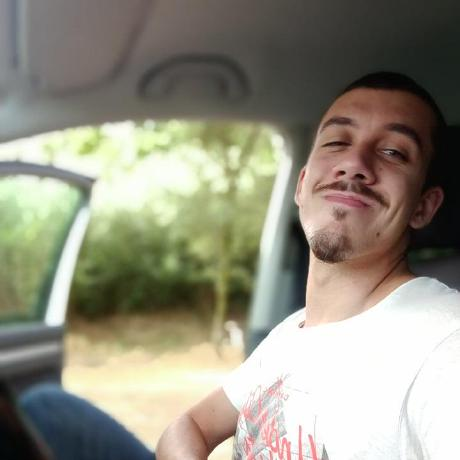
\includegraphics[height=40mm]{myfoto.jpg}}}
\end{minipage}

\textcolor{SecText}{\rule{0.9\textwidth}{0.1cm}}
\end{center}
}


\titleformat{\section}[hang]
{\Large\color{SecText}}
{}
{0em}
{\bfseries\uppercase}

\titlespacing*{\section}
{0pt}{1cm}{0.2cm}

\titleformat{\subsection}
{\bfseries}
{\hspace{-0.4em}}
{0.2em}
{}[]

\titleformat{\subsubsection}[runin]
{\normalsize\bfseries}
{}
{0em}
{\normalfont\bfseries}[ -- \hspace{1em}]

\titlespacing{\subsubsection}
{2em}{0.25em}{0em}

%Biblio
\usepackage[backend=bibtex,,doi=true,bibstyle = mla, citestyle=verbose]{biblatex}
\addbibresource{Biblio.bib}
%
\DeclareFieldFormat{doi}{%
    \small%
  \mkbibacro{DOI}\addcolon\space
  \ifhyperref
    {\href{https://doi.org/#1}{\nolinkurl{#1}}}
    {\nolinkurl{#1}}}

%==========MAIN==========
\begin{document}

%footer
\pagestyle{fancy}
\fancyfoot[LE,RO]{\textcolor{textGrey}{Avaliable at: \href{https://github.com/Pereirajpf/My_CV}{/Pereirajpf/My$\_$CV}}}
\fancyfoot[CO,RE]{\textcolor{textGrey}{\thepage}}
\fancyfoot[LO,CE]{\textcolor{textGrey}{last updated: \thedate}}
%Title box

\maketitle

%====
%Small introduction
\vspace{2mm}
\centerline{\begin{minipage}{0.85\textwidth}
\large{
\quad I'm a recent graduate in Bioinformatics with experience in \textbf{data analysis} and \textbf{programming}.\\ 
\null \quad I'm always looking for something new and exciting to learn and also available to help my colleagues in any way I can. In this new stage of my life, I'm looking for a challenge and to enhance my technical and social skills in a diverse environment.
}
\end{minipage}}

\vspace{-4mm}
%====
\section{Experience}
\vspace{-2mm}
\begin{tabular}{p{4mm} l}
\multicolumn{2}{l}{\scriptsize\textit{\textcolor{textGrey}{Jul 2020 to May 2021}}}\\
\multirow{2}*{
\includegraphics[width=1.8\linewidth]{insa_logo.jpg}} & \textbf{Research fellowship},\\
& \textit{Instituto Nacional de Saúde Doutor Ricardo Jorge (Portugal)},\\
 &\scriptsize{Grant number: Projeto nº 692 2ª edição do RESEARCH4COVID, FCT, Portugal.}\\
\end{tabular}

\vspace{-5mm}
%====
\section{Education}
\vspace{-2mm}
\begin{tabular}{L!{\VRule}R}
\small\textit{2019 - 2022} & \textbf{Master's degree in Bioinformatics and Applications to Life Sciences},\\
\multirow{2}*{
\includegraphics[width=0.4\linewidth]{utad_logo.jpg}} & \textit{University of Trás-os-Montes and Alto Douro (Portugal)},\\
& \small{Final grade: 16.}\\
[8mm]
\small\textit{2015 - 2019} & \textbf{Batcheler's degree in Biochemistry},\\
\multirow{2}*{
\includegraphics[width=0.4\linewidth]{utad_logo.jpg}} & \textit{University of Trás-os-Montes and Alto Douro (Portugal)},\\
& \small{Final grade: 13.}\\
\end{tabular}


%====
\section{Technical Skills}
\vspace{-2mm}
\subsection{\faIcon{code}  Programming}
\textcolor{textGrey}{\textbf{Intermediate knowledge}}
\subsubsection{R}
Statistical analysis, mathematical models, OOP, package development, Shiny.
\subsubsection{Python}
Statistical Analysis with Pandas, OOP, basic machine learning using TensorFlow and Keras.
\\[2mm]
\textcolor{textGrey}{\textbf{Basic knowledge}}\\
 \indent {C, Java, Matlab, SQL, Arduino.}

\subsection{\faIcon{indent}  Typesetting}
 \quad \LaTeX, Markdown.

\subsection{\faIcon{tools}  Tools}
 \quad Git and GitHub, Power BI, Hugo framework, Windows and Linux, Intermediate Microsoft Office and LibreOffice.

\subsection{\faIcon{language}  Languages}
\subsubsection{Portuguese}
native speaker
\subsubsection{English}
B2

%====
\section{Academic/Scientific work}

\subsection{\faIcon{trophy}  Distinctions}
\subsubsection{Best Poster}
Portuguese National Statistics Meeting (SPE21), Evora 2021.

%
\subsection{\faIcon{file-alt}  Publications}
\begin{tabular}{N P}
[May 2021] & Mathematical Modelling of the Impact of Non-Pharmacological Strategies to Control the COVID-19 Epidemic in Portugal;\\
& \textit{Constantino Caetano, Maria Morgado, Paula Patrício, João Pereira, Baltazar Nunes};\\
& doi:\href{https://doi.org/10.3390/math9101084}{10.3390/math9101084}\\
\end{tabular}
\\
\begin{tabular}{N P}
[Nov 2021] & The impact of vaccination on the evolution of COVID-19 in Portugall;\\
& \textit{Beatriz Machado, Liliana Antunes, Constantino Caetano, João F. Pereira, Baltazar Nunes, Paula Patrício, M. Luísa Morgado};\\
& doi:\href{https://doi.org/10.3934/mbe.2022043}{10.3934/mbe.2022043}\\
\end{tabular}
\\
\begin{tabular}{N P}
[Oct 2022] & Measuring the impact of COVID-19 vaccination and immunity waning: a modelling study for Portugal;\\
& \textit{Constantino Caetano, Maria Luísa Morgado, Paula Patrício, Andreia Leite, Ausenda Machado, André Torres, João Freitas Pereira, Sónia Namorado, Ana Sottomayor, André Peralta, Baltazar Nunes};\\
& doi:\href{https://doi.org/10.1016/j.vaccine.2022.10.007}{10.1016/j.vaccine.2022.10.007}\\
\end{tabular}
\\
\\
\textcolor{textGrey}{\textbf{Preprints}}
\\
\begin{tabular}{N P}
[Mar 2022] & COVID-19 Hospitalisation in Portugal, the first year: Results from hospital discharge data;\\
& \textit{João F. Pereira, Constantino Caetano, Liliana Antunes, Paula Patrício, Maria Luísa Morgado, Baltazar Nunes};\\
& doi:\href{https://doi.org/10.1101/2022.03.03.22271349}{10.1101/2022.03.03.22271349}\\
\end{tabular}

%
\subsection{\faIcon{archive}  Other works}

\subsubsection{Poster presentation}
\textit{Portuguese National Statistics Meeting (SPE 2021), Évora (13–16 Outubro, 2021).}\\
title: ''COVID-19 Hospitalization in Portugal: Results from hospital discharge data''\\

\subsubsection{Seminar presentation}
\textit{Ciclo de Seminários em Matemática Aplicada e Ciência de Dados (CS-MACD).}\\
title: ''Análise de dados COVID-19 em Portugal'', 7 de October 2022, UTAD.\\
link: \href{https://sites.google.com/view/cs-macd/home}{https://sites.google.com/view/cs-macd/home}\\

\subsubsection{Article review}
Scientific Reports (ISSN 2045-2322), December 2022.


\end{document}